\begin{frame}{Overdragelse og Overladelse af Våben (§ 20)}

\vspace{1em}

\begin{columns}[c] % c = center vertically

\column{0.05\textwidth} % Venstre margin

\column{0.7\textwidth} % Midten: Bullets

\small

\raggedright

\begin{itemize}

\itemsep0.3em % Justér afstand mellem bullets

\item \textbf{Hovedregel:} Våben må kun overdrages eller overlades til personer, der kan fremvise \structure{fornøden våbentilladelse}.

\item \textbf{Forskel riffel og haglvåben:} Haglvåben kan overlades til en anden person med jagttegn. Riffel må kun overdrages til person med våbentilladelse til pågældende våben.

\item \textbf{Identifikation:} Den, der modtager våbnet, skal fremvise \structure{original billedlegitimation} for at bevise, at tilladelsen tilhører vedkommende.

\item \textbf{Udlåners ansvar:} Den, der låner våbnet ud, har pligt til at kontrollere \structure{både tilladelse og legitimation}.

\item \textbf{Ungjægere:} Glatløbede haglgeværer må overlades til kursister/aspiranter af \textbf{godkendte lærere/prøvesagkyndige} i forbindelse med instruktion og prøve (§ 21).

\end{itemize}

\column{0.25\textwidth} % Højre: Ikon

\centering

\vspace{0pt}

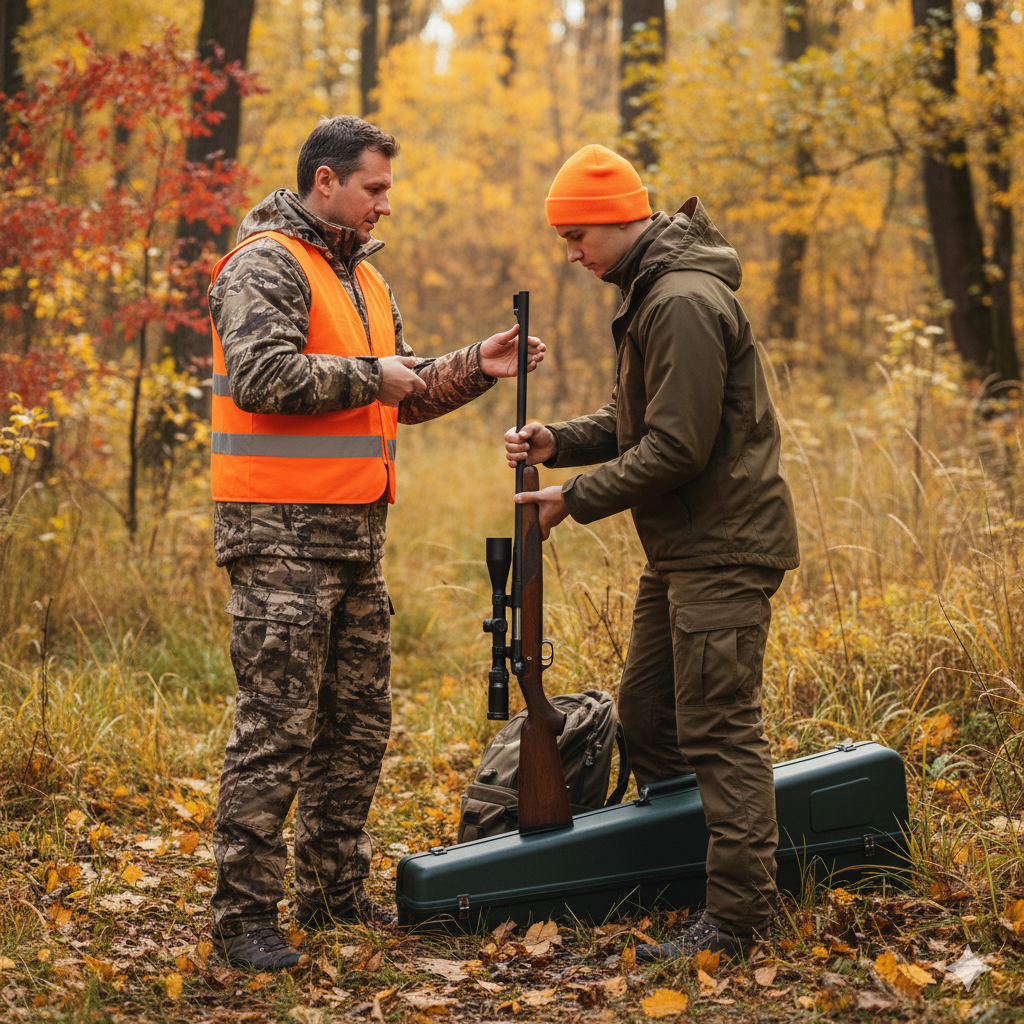
\includegraphics[width=0.9\linewidth]{Billeder/Redskaber/overdragelse.png} % Forslag til et ikon, der symboliserer overladelse/aftale

\end{columns}

\end{frame}